\chapter{如何開始撰寫自己的論文內容} \label{ch_how2start}

相信目前的文件數量仍然會讓您在評估上仍許多疑惑,
為了避免讓您在撰寫論文時遇到許多的小問題,本章將會一步步帶著您將本專案修改為您自己的論文。

\section{架構簡介}

本專案所有的設定都盡可能的模組化,讓每個目錄、檔案的操作內容皆能專注在特定的事務上。在開始之前先一一介紹本專案的架構。

\begin{itemize}
    \item Chapter - 論文各章節文件
    \item Configurations - 論文設定
    \item Docs - 專案參考文件
    \item Externals - 外部匯入文件
    \item Figures - 圖片
    \item Fonts - 字體檔案
    \item Instance - 論文文章以外的文件
    \item Packages - LaTeX package
    \item References - 參考文獻
    \item Tables - 表格
    \item Templates - 版型 sty 檔案
\end{itemize}

需要由使用者自行新增 tex 文件的目錄有 Chapter、Externals、Figures、Tables、References,這些目錄都是放置論文內容的地方,
使用者需要對陸路進行微調的目錄有 Configurations、Instance,其餘目錄則不建議變動。

\section{如何編輯}

\subsection*{Chapter 的新增、刪除、修改}

chapter 是存放內容文件的目錄,考慮到每個人的章節數量不同,因此章節載入及章節順序獨立於 Configurations/chapter.tex 中。
當然您也可以直接在一個文件中完成所有論文章節。

當您要加入一個章節,請先在 Chapters 中建立您的要新增的檔案(以下以 A.tex 作為範例)。
並在 Configurations/chapter.tex 加入這個檔案,讓編譯時被專案引入到檔案中。

\begin{lstlisting}[language=TeX]
    \input{Chapters/A.tex}
\end{lstlisting}

接著開始進行文件編輯,在邏輯上我們希望每個章節都存放在不同的 tex 檔案中,因此需要先定義此頁的章節名稱。
接著就可以開始進行論文撰寫了,如您需要更多的小節,可使用 section、subsection、subsubsection 來定義小節。

\begin{lstlisting}[language=TeX]
    \chapter{A.tex 範例01}\label{leb1}
    
    \section{小節1}
    
    \subsection{小節1-1}
    \subsection{小節1-2}
    \subsubsection{小節1-2-1}
    \subsubsection{小節1-2-2}
    \subsection{小節1-3}
    \section{小節2}
    \section{小節3}
\end{lstlisting}

當您不希望小節被加入到目錄,您可以使用 * 號來進行忽略目錄號碼。

\begin{lstlisting}[language=TeX]
    \subsection*{忽略小節號碼}
\end{lstlisting}

\subsection*{Externals、Figures、Tables}

Externals、Figures 是用來儲存匯入論文的文件、圖片用。Tables 是表格 tex 文件的儲存空間,如表格不大會建議直接將圖表直接放在 chapter 中。

匯入外部 PDF 檔案語法如下,IfFileExists 用於檢查檔案是否存在,檔案存在才會將該檔案進行引入。在編譯時引入一個不存在的檔案,將會造成編譯錯誤。
\begin{lstlisting}[language=TeX]
    \IfFileExists{Externals/ext.pdf}{
        \includepdf[pagecommand={\thispagestyle{empty}}]{Externals/ext.pdf}
    }{}
\end{lstlisting}

下方列出引入表格檔案的 tex 檔案,這個做法和加入 A.tex 到 chapter.tex 的行為相同。
\begin{lstlisting}[language=TeX]
    \input{Tables/a.tex}
\end{lstlisting}

\subsection*{Reference 修改}

本專案的 reference 工具是 bib,下面將介紹 IEEE xplore 網站的文件取得論文的 bib 的格式。

如圖\ref{fig_bib_1},在該篇論文網站的左上角,點下 Cite This 會出現如圖\ref{fig_bib_2}的視窗,切換至 BibTex 分頁即複製這份論文的 bib 語法。
再將段文字貼上到 References/reference.bib 中即可。

\begin{figure}[H] 
    \centering 
    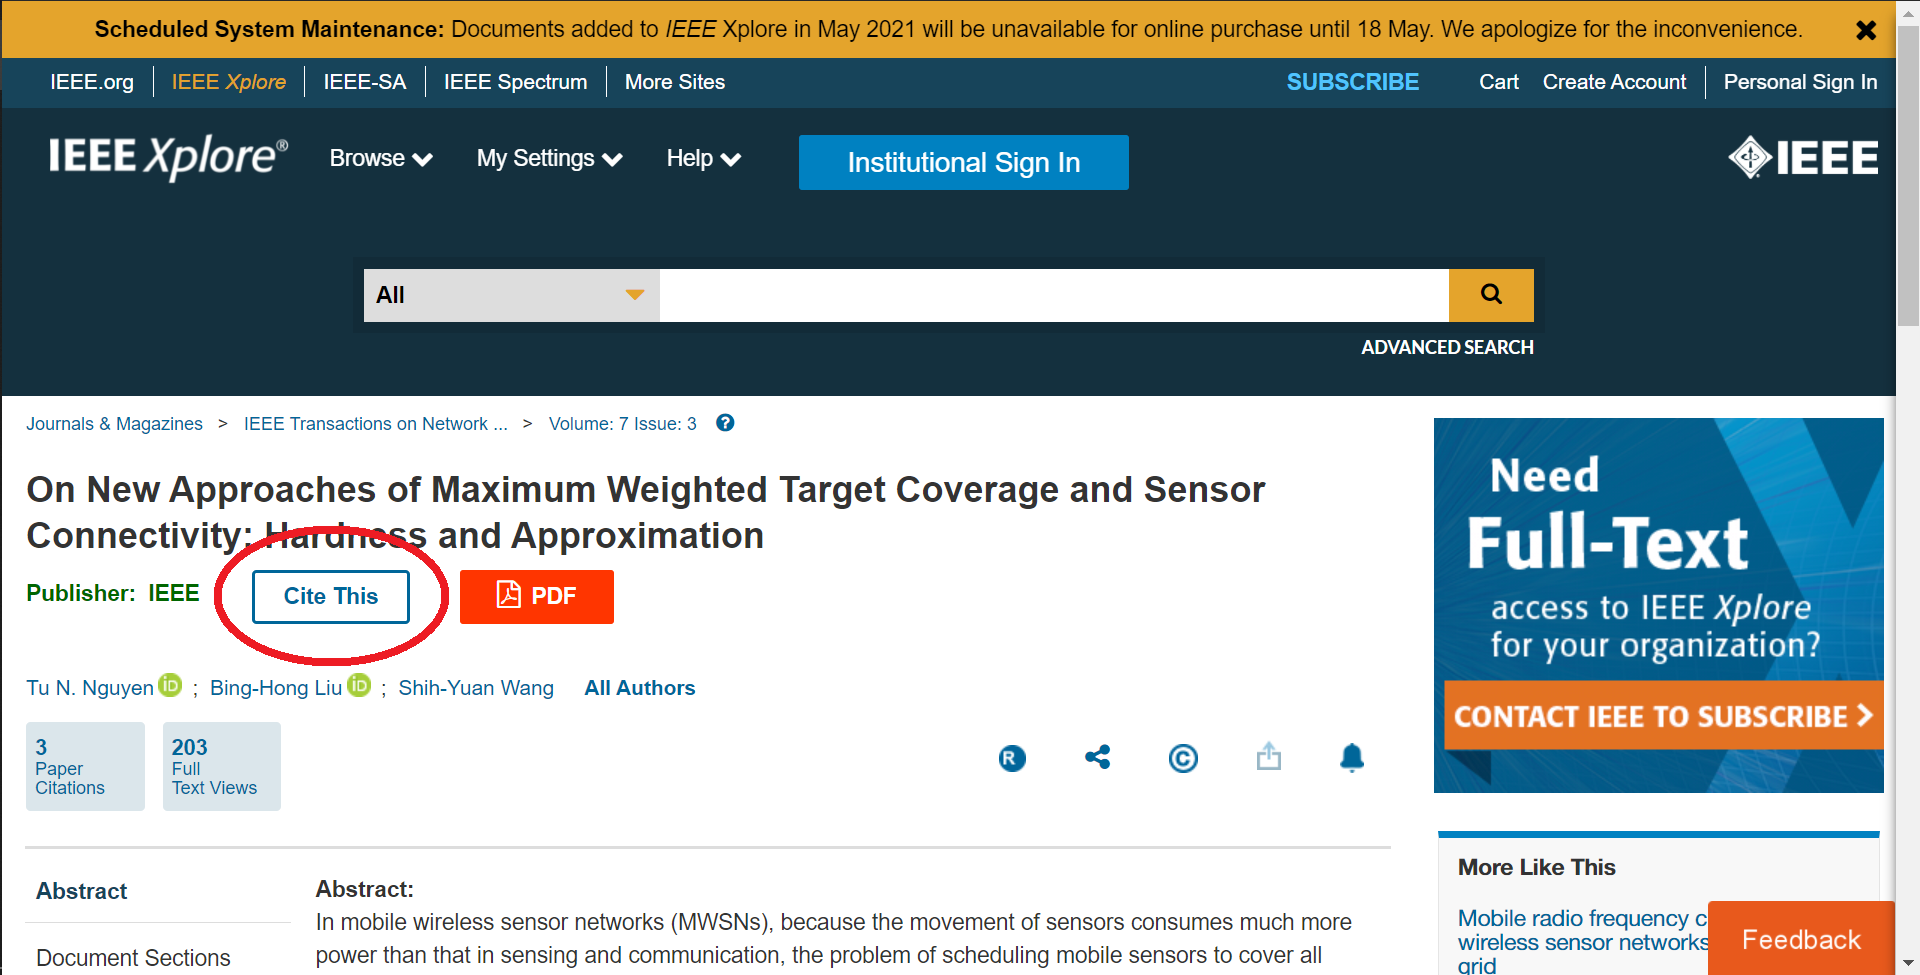
\includegraphics[width=0.5\textwidth]{./Figures/how_to_used/ieee_xplore_cite_this_bib_01.png} 
    \caption{cite this}
    \label{fig_bib_1}
\end{figure}

\begin{figure}[H] 
    \centering 
    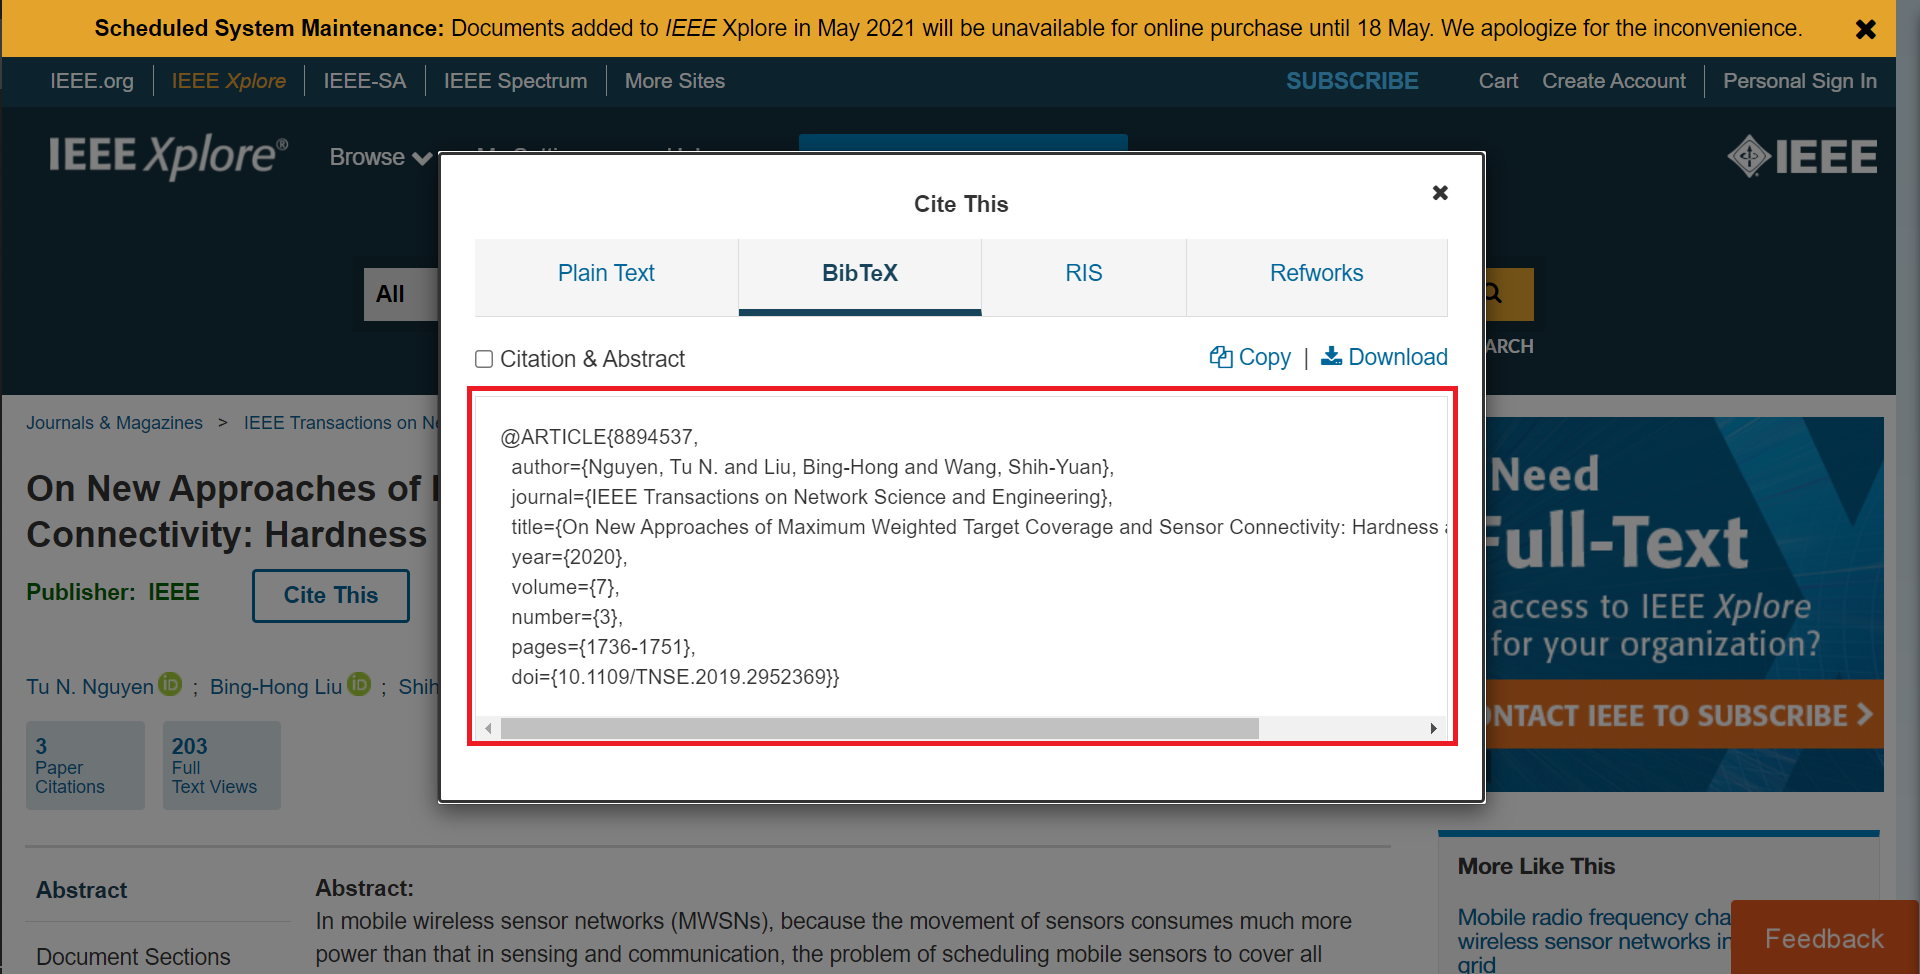
\includegraphics[width=0.5\textwidth]{./Figures/how_to_used/ieee_xplore_cite_this_bib_02.png} 
    \caption{bibtex text}
    \label{fig_bib_2}
\end{figure}
